\documentclass[12pt,a4paper]{styles/report}
\usepackage{mathtext}
\usepackage[T2A]{fontenc}
\usepackage[utf8x]{inputenc}
\usepackage[english, russian]{babel}
\usepackage{textcase}

\usepackage{graphics}
\usepackage{graphicx}
% ����� ��� ����������� ����������� � ���������� � �� ������� \cite � \ref
\usepackage{hyperref}
\usepackage{latexsym}
\usepackage{styles/axodraw}
\usepackage{indentfirst}
\usepackage{cite}
\usepackage{styles/caption-disser}
%\usepackage{flafter}
\usepackage{float}
% ���� ����� ������ ������������ ��� �������� ������ �� ����������
%\usepackage{amsbib}


% ���������� �������� �������� ������ � ���� �������
% !!!!!!!  ����� ������� ������ !!!!!
%\usepackage{showkeys}

% ������ ���������� ��� �������� ����� �������
\frenchspacing

\oddsidemargin=5mm \topmargin=-10mm \headheight=0mm \headsep=0mm
\footskip=10mm \textheight=255mm \textwidth=165mm


\newcommand{\dd}{\mbox{{\rm d}}}
\newcommand{\half}{{\textstyle\frac{1}{2}}}
\newcommand{\third}{{\textstyle\frac{1}{3}}}
\newcommand{\fourth}{{\textstyle\frac{1}{4}}}
\def\lsim{\mathrel{\rlap{\raise 2.5pt \hbox{$<$}}\lower 2.5pt
\hbox{$\sim$}}}
\newcommand{\wmax}{w_{\rm max}}
\renewcommand{\Re}{\mbox{Re}}
\newcommand{\thW}{\theta_{{\rm W}}}
\newcommand{\varepsilonmax}{\varepsilon_{\rm max}}
\newcommand{\Tr}{{\rm Tr}}
\newcommand{\kslash}{\rlap/k}
\newcommand{\qslash}{\rlap/q}
\newcommand{\Order}{{\cal O}}
\newcommand{\TeV}{{\rm TeV}}
\newcommand{\Lumint}{{\cal L}_{\rm int}}


\usepackage[dvips]{color}
\definecolor{Black}{named}{Black}
\definecolor{Red}{named}{Red}
\definecolor{Blue}{named}{Blue}
\newcommand{\black}[1]{\color{Black} #1\color{Black}}
\newcommand{\red}[1]{\color{Red} #1\color{Black}}
\def\change#1{{\red{\sl #1}}}
\def\comment#1{{\small \red{[{\sl #1}]}}}
\newcommand{\blue}[1]{\color{Blue} #1\color{Black}}
\def\change#1{{\blue{\sl #1}}}
\def\comment#1{{\small \blue{[{\sl #1}]}}}

\emergencystretch=30pt

\righthyphenmin=2


%\bibident=0pt

\begin{document}
	
\renewcommand\contentsname{СОДЕРЖАНИЕ}
\renewcommand{\bibname}{СПИСОК ИСПОЛЬЗОВАННЫХ ИСТОЧНИКОВ}
\renewcommand\chaptername{ГЛАВА}
\renewcommand\figurename{Рисунок}
\renewcommand\tablename{Таблица}

%%%%%%%%%% Титульный лист
\begin{titlepage}
	\large
	\begin{center}
		\vspace{3mm}
		МИНИСТЕРСТВО ОБРАЗОВАНИЯ РЕСПУБЛИКИ БЕЛАРУСЬ\\
		УЧРЕЖДЕНИЕ ОБРАЗОВАНИЯ\\
		«Гомельский государственный технический университет имени П.О. Сухого»\\
		\vspace{10mm}
		КАФЕДРА «ИНФОРМАЦИОННЫЕ ТЕХНОЛОГИИ»\\
		\vspace{30mm}
		РЕФЕРАТ\\
		на тему\\
			\textbf{\MakeTextUppercase{ Программный комплекс для имитационного моделирования рождения $Z^\prime$ - бозонов в протон-протонных столкновениях с учетом эффектов $Z$ - $Z^\prime$ смешивания
		}}\\
	\vspace{5mm}
		подготовленный для прохождения итоговой аттестации 
		по общеобразовательной дисциплине 
		<<Основы информационных технологи>>\\
	\vspace{40mm}
		Выполнил:\\
		магистрант гр. МАГ 40-22
		специальности 1–40 80 04 <<Математическое моделирование, численные методы и комплексы программ>>\\
		Бурим Илья Павлович
		
	\vspace{15mm}
		Проверил:\\
		доцент кафедры <<Информационные технологии>>\\
		Цитринов А.В.
	\vfill
		Гомель 2017
	\end{center}
\end{titlepage}
%%%%%%%%%%%%%%%

\newpage
\pagestyle{plain} \pagenumbering{arabic} \setcounter{page}{2}
\large \tableofcontents

%\chapter*{ВВЕДЕНИЕ}
\addcontentsline{toc}{chapter}{ВВЕДЕНИЕ} % in Content
Одной из основных задач современной теоретической и экспериментальной физики является проверка Стандартной модели электрослабых и сильных взаимодействий элементарных частиц (СМ)~\cite{2part-1}, которая осуществлялась в ускорительных экспериментах на высокоэнергетических коллайдерах, таких как \textit{LEP}, \textit{SLC}, \textit{Tevatron}, \textit{HERA} и др.~\cite{sirunyan:2017}, а также интенсивно ведется в настоящее время на Большом адронном коллайдере \textit{LHC}~\cite{main-book}. Последний громкий успех СМ связан с открытием хиггсовского бозона в экспериментах CMS и \textit{ATLAS} на \textit{LHC}~\cite{Krasnikov:2004}. Для более детального исследования свойств хиггсовсого бозона планируются новые коллайдерные эксперименты, такие как проекты \textit{ILC} и \textit{CLIC}~\cite{2part-pankov}. Стандартная модель не объясняет, что такое гравитация и как она связана с другими силами и частицами. Также она не объясняет, почему основными частицами вещества являются кварки и лептоны и сколько их должно быть. Кроме этого Стандартная модель не объясняет таких явлений, которые по праву должны учитываться при больших энергиях, а теперь исследуются ускорителями частиц. Одно их таких явлений – «темная материя». По последним данным считается, что доминирующей формой материи во Вселенной является так называемая «Темная материя». Без темной материи галактики и звезды не сформировались бы и жизни не существовало бы. Только в последние 10-15 лет ученые добились существенного прогресса в понимании свойств темной материи. Недавние наблюдения влияния темной материи на структуру Вселенной показали, что она отличается от любой формы материи, которую обнаружили или измерили в лаборатории. В то же время появились новые теории, которые могут сказать нам, что такое темная материя. В настоящее время на современных ускорителях элементарных частиц ведутся поиски кандидатов на частицы темной материи. Если эти частицы имеют массы, которые измеряются в шкале ТэВ, то они могут быть обнаружены на Большом адронном коллайдере. Однако проверка того, что эти новые частицы действительно связаны с темной материей, потребует, получение их характеристик~\cite{nuclphys:weak}.

Экспериментальные программы физических экспериментов уже завершенных коллайдерных исследований (\textit{LEP}, \textit{TEVATRON}, и др.), текущих экспериментов (Большой адронный коллайдер -- Швейцария, Франция), строящихся (\textit{NICA} -- Россия) и планируемых в ближайшем будущем экспериментов (Международный линейный электрон-позитронный коллайдер в Японии; \textit{CLIC} -- Швейцария, Франция) содержат разделы, посвящённые исследованиям моделей новой физики, выходящим за рамки Стандартной модели элементарных частиц. В том числе, эти программы физических экспериментов включают в себя задачи по поиску эффектов новых ${Z}^{\prime}$-бозонов и получению ограничений на параметры ${Z}^{\prime}$-бозонов. Поэтому задача оценки ограничений на углы смешивания и массу ${Z}^{\prime}$-бозонов в условиях экспериментов на Большом адронном коллайдере является актуальной.

В силу вероятностной природы процессов взаимодействия элементарных частиц, имитационное моделирование является одним из главных инструментов для моделирования результатов текущих и планируемых экспериментов в физике элементарных частиц и высоких энергий. В настоящее время, имитационное моделирование широко применяется для моделирования фоновых событий для очистки экспериментальных данных а также для моделирования эффектов новой физики.

%В настоящей работе имитационное моделирование использовано для моделирования  эффектов $Z-{Z}^{\prime}$ смешивания в процессе $pp \rightarrow W^+W^- + X$ в условиях экспериментов на Большом адронном коллайдере и анализа экспериментальных данных Большого адронного коллайдера с целью получения оценок (ограничений) на параметры ${Z}^{\prime}$-бозонов: углы смешивания и массу ${Z}^{\prime}$-бозонов.


\chapter{Рождения $Z^\prime$ - бозонов в протон-протонных столкновениях с учетом эффектов $Z$ - $Z^\prime$ смешивания}
Многие сценарии Новой Физики (НФ) отличной от Стандратной Модели (СМ)~\cite{2part-1}, включая модель суперпозиций и левую-правую симметричную модель, предсказывают существование новых нейтральных и заряженных калибровочных бозонов, которые могут быть найдены на текущих или будущих коллайдерах. Поиск нового нейтрального $Z^\prime$ и заряженного $W^\prime$ калибровочных бозонов является важным аспектом экспереметально-физических программ на колладерах больших энергий. В этой работе сконцентрировано внимание на первом бозоне.

Предоставленные лимиты большого адронного коллайдера и виртуальные эффекты ЛЭП, через интерференцию или смешивания с $Z$ бозонами, подразумевает что любые $Z^\prime$ бозоны горазда тяжелее и менее смешиваются с $Z$ бозонами. В зависимости от рассматриваемой теоретической модели $Z$ массы порядка 4,5 ТэВ~\cite{2part-pankov} и $Z-Z^\prime$ углов смешивания на уровне нескольких градусов исключены~\cite{sirunyan:2017}. Угол смешивания сильно ограничен очень высокоточными экспериментами на ЛЭП и \textit{SLC}. Они включают в себя измерения из формы линии \textit{Z}, из лептонных отношений ветвления, нормированных на общую адронную ширину затухания $Z$, а также от лептонных лево-правых асимметрий. $Z^\prime$, легче чем 5 ТэВ, может быть обнаружен на БАК~\cite{sirunyan:2017} c $\sqrt{s} = 14 $ ТэВ в процессе Дрелл-Янга (ДЯ) $pp \rightarrow Z^\prime \rightarrow l^+l^- + X$, где $l=e,\mu$.

После открытия $Z^\prime$-бозона на БАК через процесс ДЯ, необходимо произвести некоторую диагностику связей и смешивания $Z$-$Z^\prime$, чтобы идентифицировать основную теоретическую структуру. В настоящей работе исследуются данные \textit{ATLAS}~\cite{main-book} и \textit{CMS} в канале дибозона:

\begin{equation} \label{eq:1}
pp \rightarrow W^+W^- + X.
\end{equation}

Для поиска \textit{Z}-бозона, который возникает, например, в популярной модели с расширенным калибровочным сектором~\ref{eq:1}. Анализ основан на данных о столкновениях $pp$ при энергии центра масс $\sqrt{s} = 13 $ собранных группами \textit{ATLAS}~\cite{main-book} и \textit{CMS} на БАК. В частности, данные используются для поиска $Z$-$Z^\prime$ смешивание. На \textit{ATLAS} события $W^+W^-$ реконструируются через их полулептонные распады $W$, где один $W$-бозон распадается на заряженный лептон ($l=e,\mu$) и нейтрино, а другой на две струи, тогда как на CMS $W$-бозон адронически распадается на две восстановленные струи. 

Процесс рождения пары $W^-W^+$-бозонов~\ref{eq:1} важен для изучения электрослабой калибровочной симметрии. Общие свойства слабых калибровочных бозонов тесно связаны с нарушением электрослабой симметрии и структуры калибровочного сектора, как и существование и структура трилинейных связей. Кроме того, канал распада дибозонов $Z^\prime$ исследует толщину калибровочной связи между новым и калибровочными бозонами стандартной модели. Кроме того, сила связи очень влияет на элементы распада и естественную ширину такого нового калибровочного бозона. Таким образом, детальное рассмотрение процесса~\ref{eq:1} с высокой точностью проверяет калибровочный сектор СM и может пролить свет на бозоны, которые могут появиться за пределами СМ. Здесь мы рассмотрим возможность наблюдения $Z^\prime$-бозона в $W^+W^-$ парного процесса на БАК, который в отличие от процесса ДЯ не является основным каналом поиска, но может помочь понять происхождение новых калибровочных бозонов.

Поиски тяжелого \textit{WW} резонанса были выполнены на Теватроне исследовательскими группами \textit{CDF} и \textit{D0}. Группа \textit{D0} изучала резонансное рождение дибозонов до 700 ГэВ в каналах распада $lvl^\prime v^\prime$ и $lvjj$~\cite{Krasnikov:2004}. Группа \textit{CDF} также исследовала резонанс в $WW$ в канале распада $evjj$, что в результате привело к обнаружения нижних лимитов масс $Z^\prime$
и $W^\prime$-бозонов, за исключением масс превышающих 900 ГэВ, зависящих от параметра смешивания.

Исследования \textit{WW}-резонансов группами \textit{ATLAS} и \textit{CMS} с использованием, соответственно, полулептонных и адронных событий распада в $pp$ столкновениях при 13 ТэВ устанавливают массовые пределы 3 ТэВ для этих резонансов~\cite{nuclphys:weak}. 

В диссертационной работе изучается возможность рождения нового резонанса нейтрального спина 1 ($Z^\prime$) из доступных данных групп \textit{ATLAS} для $W^+W^-$ распадов. В качестве результатов работы будут получены ограничения на соответствующие $Z-Z^\prime$-коэффициенты смешивания и на массу $M_{Z^\prime}$.
Выполнено моделирование событий рождения $Z^\prime$ бозонов в процессе распада на фотонную пару и моделирование событий рождения гравитонов в процессе $lvl^\prime v^\prime$. Создано \textit{web}-приложение для демонстрации результатов вычисления.

Несмотря на впечатляющий успех в описании экспериментов, Стандартная модель не может считаться окончательной теорией элементарных частиц. У нее есть свои трудности. Физики уверены, что она должна быть частью некоторой более глубокой теории строения микромира, той частью, которая видна в экспериментах на коллайдерах при энергиях ниже примерно 1 ТэВ. Главная задача Большого адронного коллайдера — получить хотя бы первые намеки на то, что это за более глубокая теория.

Теоретики разработали большое число кандидатов на такую теорию. Все они, естественно, включают какие-то элементы, которые отсутствуют в Стандартной модели. Часто такие теории коллективно называют «Новая физика» или «За пределами Стандартной модели». На этой странице перечислены некоторые из активно изучаемых вариантов Новой физики~\cite{2part-1}.

\begin{figure}[h]
	\centering
	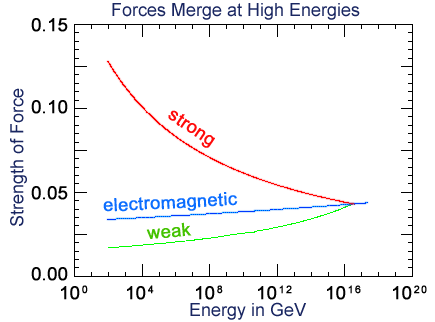
\includegraphics[width=\textwidth]{figures/hep-sm.png}
	\caption{Константы связи трех типов взаимодействий}
	\label{fig:fig01}
\end{figure}

Суперсимметрия -- это гипотетическая симметрия между фермионами и бозонами. Теории, использующие эту идею, оказываются удивительно мощными, и потому именно с суперсимметрией многие связывают надежды на открытие физики за пределами Стандартной модели. Однако до сих пор не было получено ни одного убедительного доказательства в пользу того, что суперсимметрия реализуется в нашем мире. Ее поиск является одной из главных задач Большого адронного коллайдера.

Константы связи трех взаимодействий частиц в микромире сходятся к одному значению, если имеющиеся сейчас данные экстраполировать в область очень высоких энергий. Это совпадение считается неслучайным и воспринимается физиками как намек на то, что все три взаимодействия при больших энергиях объединяются в одно.

В XIX веке физики обнаружили, что электричество и магнетизм — это две стороны одной медали, электромагнитного взаимодействия. Век спустя, при создании Стандартной модели, электромагнетизм и слабые ядерные силы были объединены в рамках единого электрослабого взаимодействия. Точнее говоря, внутри электрослабого взаимодействия имеются по-прежнему две разные силы, а электромагнитное и слабое взаимодействия возникают как комбинации этих сил. Каждое такое объединение упрощало теорию, уменьшало количество введенных в нее «сущностей», переводило наше понимание микромира на новый уровень.

Сейчас физики имеют сразу несколько причин подозревать, что при очень высоких энергиях происходит объединение электрослабого и сильного взаимодействий (рисунок~\ref{fig:fig01}). Модели, использующие эту идею (так называемые Теории великого объединения) разрабатываются уже давно. В идеале хотелось бы, чтобы такая теория естественным образом объясняла, почему фундаментальных взаимодействий именно столько и именно с такими свойствами, а также имела четкие предсказания, доступные проверке в современных экспериментах~\cite{main-book2}.

При энергиях элементарных частиц, доступных на ускорителях, гравитация по-прежнему остается исключительно слабой, так что заметить ее проявления не удается. Однако ее сила растет с ростом энергии, и при энергиях столкновения порядка планковской она станет столь же важной, как и другие взаимодействия. В этом случае в полный рост встает исключительно сложный вопрос о том, как включить гравитацию в квантовое описание микромира. Поскольку гравитация в современной физике считается проявлением кривизны пространства-времени, успешная теория с сильной гравитацией должна описывать в рамках единого формализма не только все взаимодействия и всё вещество, но и структуру пространства-времени.

Одним из наиболее привлекательных путей решения этого вопроса является теория суперструн и ее дальнейшее развитие в виде теории бран и М-теории. В этих теориях считается, что фундаментальными объектами, существующими в многомерной вселенной, являются не точечные частицы, а протяженные объекты -- струны, мембраны и еще более многомерные образования. В этой теории были получены впечатляющие успехи при высоких энергиях, однако при попытке вывести свойства нашего низкоэнергетического мира из теории суперструн возникает обескураживающая неопределенность предсказаний.

Долгое время казалось, что проверка предсказаний теории суперструн лежит далеко за пределами возможностей человечества, поскольку речь идет об энергиях, на 15 порядков превышающих энергии современных ускорителей. Однако примерно 10 лет назад возникло новое направление развития теории, в котором гравитация становится сильной на энергиях порядка 1 ТэВ. Такая возможность возникает в том случае, если наш мир более чем трехмерный и если при этом новые дополнительные пространственные размерности достаточно протяженны: либо они бесконечны, либо свернуты в многомерные петельки размером много больше ядерного масштаба.

В этом случае на \textit{LHC} следует ожидать целый ряд совершенно замечательных эффектов, отсутствующих в Стандартной модели, например, рождение гравитонов, которые будут улетать из нашего мира в дополнительные измерения, и микроскопических черных дыр, тут же испаряющихся с испусканием множества обычных частиц. Будут также наблюдаться сильные отклонения от предсказаний Стандартной модели в столкновении обычных частиц. Стоит, впрочем, подчеркнуть, что пока нет никаких экспериментальных подтверждений того, что эта красивая гипотеза имеет отношение к нашему миру.

Все три перечисленные выше направления «Новой физики» опираются на глубокие теоретические гипотезы об устройстве нашего мира (суперсимметрия, единство сил, квантово-гравитационная вселенная). Однако кроме этих направлений теоретики также рассматривают разнообразные теории «статусом пониже». В этих теориях просто отмечается, что текущие экспериментальные данные не запрещают те или иные экзотические объекты или явления, и разрабатываются их следствия. Вот несколько примеров таких моделей разной степени экзотичности.

Неминимальные хиггсовские модели. Поскольку хиггсовские бозоны — единственные частицы Стандартной модели, до сих пор не открытые экспериментально, теоретики изучают самые разные варианты устройства этого сектора теории.
Новые поколения фермионов. Можно предположить, что кроме трех известных поколений кварков и лептонов существуют и другие поколения. Частицы из этих поколений должны быть очень тяжелыми, иначе бы их уже давно открыли в эксперименте.

Новые короткодействующие силы. В таких моделях предполагается, что в нашем мире есть и иные силовые взаимодействия, отличные от сильных, слабых и электромагнитных, но они настолько короткодействующие, что до сих пор никак не проявлялись в эксперименте. На Большом адронном коллайдере благодаря его рекордной энергии удается «прощупать» взаимодействия частиц на исключительно малых расстояниях (менее 10–19 метра), а значит, появляется шанс эти взаимодействия обнаружить. Они могут проявляться либо как рождение и распад частицы-переносчика новых сил (такие гипотетические частицы обозначают $Z^\prime$), либо как усиленное рассеяние частиц на большие углы.

\begin{figure}[h]
	\centering
	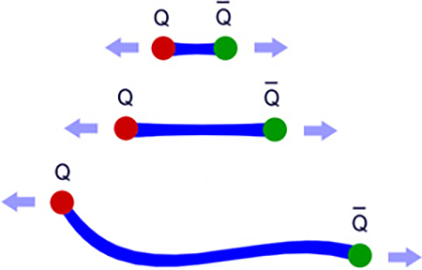
\includegraphics[width=\textwidth]{figures/quirk-antiquirk.jpg}
	\caption{Кварки}
	\label{fig:fig03}
\end{figure}

Лептокварки. В Стандартной модели и в подавляющем большинстве теорий Новой физики кварки и лептоны взаимодействуют друг с другом опосредованно, путем обмена квантами силовых полей. Однако можно представить себе возможность того, что кварки и лептоны исходно являлись фермионами одного типа и лишь потом расщепились на два разных сорта. В таком случае должны существовать новые тяжелые частицы — лептокварки, которые распадаются прямо на кварк и лептон. Подобные частицы встречаются в теориях Великого объединения.

Квирки. Одним из очень необычных и любопытных вариантов новых сил является гипотеза квирков (\textit{quirks}). Эта модель построена по типу обычного сильного взаимодействия: в ней предполагается, что существует новое силовое поле с конфайнментом и новые частицы, его чувствующие. Если частицы очень тяжелые, то между ними будут натягиваться длинные, даже макроскопические силовые струны, которые не смогут порваться (рисунок~\ref{fig:fig03}).

Слабое взаимодействие – короткодействующее фундаментальное взаимодействие между элементарными частицами, ответственное за бета-распад атомных ядер и медленные распады частиц. Слабое взаимодействие значительно слабее сильного и электромагнитного, но гораздо сильнее гравитационного. В слабом взаимодействии участвуют все фундаментальные фермионы (кварки и лептоны) и все адроны. Единственными частицами, которые участвуют только в слабом взаимодействии являются три типа нейтрино $v_e$, $v_\mu$, $v_\tau$ и их античастицы  антинейтрино $\bar{v_e}$,  антинейтрино $\bar{v_\mu}$,  антинейтрино $\bar{v_\tau}$. В нем не участвуют переносчики сильного, электромагнитного и гравитационного взаимодействий -- глюон, фотон и гравитон. В процессе слабого взаимодействия частицы обмениваются переносчиками слабого взаимодействия промежуточными (фундаментальными) бозонами: имеющими электрический заряд $W^±$ и нейтральным $Z$. Эти бозоны, в отличие от переносчиков остальных фундаментальных сил безмассовых глюона, фотона и гравитона, имеют огромные массы $m_W$ = 80.4 ГэВ/с~${}^2$ и $m_Z$ = 91.2 ГэВ/с${}^2$ (примерно как у атомов циркония или ниобия), что приводит к очень малому радиусу действия слабых сил ≈10-18 см (что на три порядка меньше радиуса сильного взаимодействия) и очень низкой по сравнению с сильными и электромагнитными процессами вероятности (скорости) слабых процессов.

Несмотря на малую величину и короткодействие слабые силы играют очень важную роль в природе. Так без них погасло бы Солнце, так как внутри него остановился бы процесс превращения 4 протонов в ядро гелия-4, являющийся основным источником энергии Солнца.

Слабое взаимодействие выделяется тем, что в нём не соблюдается ряд запретов, присущих сильному и электромагнитному взаимодействиям. Так в слабых процессах кварки одного типа (аромата) превращаются в кварки других ароматов~\cite{nuclphys:weak}.

Особенности слабого взаимодействия:
\begin{enumerate}
	\item[--] их слабость (медленность), выражающаяся в том, что
	вероятность этих процессов на много порядков меньше
	вероятностей сильных и электромагнитных процессов;
	
	\item[--] малый радиус взаимодействия —как минимум на
	два порядка меньший, чем радиус сильного взаимодействия.
	Ни в одном из слабых процессов не удалось до 1982 г. обнаружить каких-либо отклонений от точечного четырех-
	фермионного взаимодействия;
	
	\item[--] сильное, максимально возможное несохранение пространственной и зарядовой четностей. Так, в заряженные
	токи входят только левые компоненты спиноров, описывающих частицы, и только правые компоненты спиноров,
	описывающих античастицы;
	
	\item[--] несохранение \textit{СР}-четности;
	
	\item[--] несохранение ароматов (странности, чарма и т. д.);
	
	\item[--]  то обстоятельство, что только в слабых взаимодействиях принимают участие нейтрино.
	
\end{enumerate}

Тем поразительней, что, несмотря на столь резкие отличия, слабые и электромагнитные взаимодействия представляют собой, по-видимому, проявление одного и того же
взаимодействия, которое в последние годы получило название электрослабого.

Согласно электрослабой теории слабые взаимодействия
заряженных токов обусловлены обменами $W$-бозонами, а
нейтральных -- $Z$-бозонами, подобно тому как взаимодействие электромагнитных токов обусловлено обменом фотонами. При этом слабость и малый радиус слабого взаимодействия объясняются тем, что, в отличие от фотонов, $W$ и $Z$-бозоны -- очень тяжелые частицы Остальные особенности слабого взаимодействия прямо заложены в предположении о форме исходных фермионных токов теории.
Так что в злектрослабой теории удивляться надо не тому,
что слабое взаимодействие зеркально-асимметрично, a тому, что электромагнитное -- зеркально-симметричное.

Слабое взаимодействие переносится массивными $W^±$- и $Z$-бозонами. Обмен заряженными $W^+$ и $W^-$-бозонами приводит к изменению электрического заряда взаимодействующих фермионов. Эти процессы происходят за счет заряженных токов.





\section{Инструменты имитационного моделирования}

Физика высоких энергий — передовое направление современной науки, конечной целью которого является открытие наиболее фундаментальных законов микромира, управляющих эволюцией материи во Вселенной, начиная с момента ее рождения при Большом взрыве. Физика высоких энергий встречает XXI век реализацией гигантского проекта Большого адронного коллайдера (БАК)~\cite{2part-1}. Этот уникальный, не имеющий себе равных по масштабам и сложности, научный проект, который находится сейчас в процессе реализации международным сообществом физиков из более чем 40 стран на базе европейской организации ядерных исследований, базирующейся в Женеве, направлен на решение краеугольных проблем современной субъядерной физики.

Для исследования отклика детектора на различные физические процессы, созданы программы, позволяющие перевести моделированное на уровне частиц событие  взаимодействия протонов при соударении в формат представления данных детекторов установки \textit{ATLAS}. Алгоритмы моделирования интегрированы в программную оболочку эксперимента  \textit{ATLAS}, именуемую \textit{Athena}, использующую программный пакет \textit{GEANT4}.

Генератор события создает набор частиц, который направляется в программу быстрого или полного моделирования детектора. Генераторы событий встроены в \textit{Athena}. Используется большое число других, поддерживаемых авторами, генераторов, которые имеют блоки связи для использования в \textit{Athena}. Основной массив модельных событий создан с помощью генераторов \textit{PYTHIA}~\cite{2part-pythia-all}, включая его версию \textit{PYTHIAВ},  предназначенную в  \textit{ATLAS} для моделирования событий с рождением \textit{В}-адронов.

\textit{PYTHIA} - это программного пакета для визуализации результатов моделирования процессов столкновения частиц при высоких энергиях осуществляющего генерацию методом Монте-Карло физических событий.

Программы \textit{PYTHIA} интенсивно используются для генерации событий в физике высоких энергий при описании процессов множественного рождения в столкновениях элементарных частиц. В частности задачи, что включает решаемые жесткие с взаимодействия помощью данного в столкновениях $e^+e^-$, $pp$ и $ep$, а также некоторые другие случаи. Программа предназначенна для генерации генератора полных событий, т.е. дают более детальную картину, чем мы наблюдаем в эксперименте, в рамках нашего понимания фундаментальной физики процессов. Обсуждаемые здесь программы Монте-Карло построены как ведомые системы, т.е. пользователь должен написать основную программу. Из нее различные программы вызываются для выполнения частных задач, после чего управление снова передается основной программе. Некоторые из этих задач могут быть весьма тривиальными, и достаточно высокоуровневые программы могут производить большое число вызовов подпрограмм.

Генераторы общего назначения создают событие как целое. Они используют много параметров, часть из которых относится к фундаментальным параметрам, такие как константы связи квантовой хромодинамики (КХД) и электрослабой теории, часть относится к моделям, описывающим взаимодействия на больших расстояниях, с малыми передачами импульса, т.н. «мягкой» КХД, и к электрослабым процессам.

Для корректного моделирования процессов рождения и распада частиц необходимо учитывать условия проведения эксперимента. Это условия рождения изучаемых частиц на ускорителе при соответствующих энергиях сталкивающихся пучков, полные цепочки распадов частиц до уровня <<стабильных частиц>>, регистрируемых детектором. Для решения этих задач применяются генераторы событий, использующие метод Монте-Карло.
Генератор \textit{PYTHIA} является широко используемой в физике высоких энергий программой моделирования столкновений различных частиц в широком диапазоне энергий. Этот генератор учитывает процессы фрагментации кварков в адроны и разыгрывает сложные цепочки адронных распадов. Стартуя с заданного пользователем процесса, (столкновение двух протонов с рождением \textit{Z}-бозона и т.п.) программа случайным образом (с учетом законов сохранения и, по возможности, теоретически известной структуры взаимодействия) разыгрывает конфигурацию конечных партонов, а затем моделирует т.н. процесс адронизации - процесс превращения ненаблюдаемых кварков и глюонов в реальные стабильные и нестабильные частицы с последующим распадом нестабильных частиц. На выходе программа выдает список всех частиц, родившихся в результате столкновения заданных первичных частиц, значения их компонент импульса и энергии. Кроме того, имеется возможность проследить последовательность рождений и распадов от первичного взаимодействия до рождения данной частицы. В качестве входных параметров программы используются описания сталкивающихся частиц, их энергий и тип моделируемого процесса (например, рождение \textit{Z}-бозона). Существующие версии пакета \textit{РYTHIА} написаны на языке программирования \textit{FORTRAN}.
Результаты генерации -- характеристики вторичных частиц -- записываются в файл, что позволяет в дальнейшем проводить статистическую обработку событий.
В физических программаx экспериментов на  современных  дронных (\textit{LHC}) и планируемых на  электрон-позитронных (\textit{ILC, CLIC}) коллайдерах вопросу поиск  <<новой>> физики, выходящей за  рамки Стандартной модели (СМ), традиционно уделяется большое внимание. К числу подобных теоретических построений, являющихся обобщением СМ, относятся модели с расширенным к либровочным сектором, такие как лево-правосимметричные модели (\textit{LR}), альтернативные лево-правосимметричные модели (\textit{ALR}), $E_6$-модели
и др.~\cite{Bobovnikov:2016}. Их исследование (теоретическое и экспериментальное) представляет значительный интерес. Эти модели являются одними из простейших расширений СМ, характеризующихся элементарной структурой хиггсовского сектора. Общим для данных моделей является то, что они предсказывают новые физические объекты и явления на масштабе энергий $O$ (1 ТэВ), связанные, например, с наличием тяжелых нейтральных ($Z^\prime$) калибровочных бозонов, обусловленных дополнительными калибровочными симметриями $U(1)^\prime$.

Достижение порога рождения $Z^\prime$-бозона явилось бы прямым доказательством проявления «новой» физики. Однако в данном случае интервал поиска масс $Z^\prime$ ограничен максимальной энергией коллайдера, на котором проводятся эксперименты. Значительно более широкий интервал масс можно исследовать с помощью пропагаторных эффектов. В этом случае ведется поиск отклонений различных наблюдаемых от соответствующих предсказаний СМ. Если экспериментальные данные при достигнутом уровне точности согласуются с СМ, т. е. отклонений от предсказаний СМ нет, то эту экспериментальную информацию можно использовать для получения ограничений на динамические параметры и массы $Z^\prime$-бозонов.

Потенциальные возможности $e^+$$e^-$-коллайдеров для прямого рождения новых калибровочных бозонов гораздо скромнее по сравнению с адронными машинами из-за более низких энергий пучков. Кроме того, современные ограничения на массы $Z^\prime$-бозонов для большинства моделей превосходят планируемую энергию электрон-позитронного коллайдера \textit{ILC}, $\sqrt{s}<< M_{Z^\prime}$. Тем не менее основным достоинством этих машин является возможность проведения экспериментов по измерению наблюдаемых величин с высокой степенью точности и получения однозначной информации о косвенных (виртуальных) эффектах новых $Z^\prime$-бозонов, а также эффектах бозонного $Z$-$Z^\prime$-смешивания. Последние, в моделях с расширенным калибровочным сектором, зависят от структуры хиггсовского сектора модели. Тем самым экспериментальное исследование процессов рождения пар $W^±$-бозонов может не только пролить свет на возможное существование <<новой>> физики, но и дать косвенные указания на хиггсовскую природу, а также установить структуру модели.

На основе данных, полученных из низкоэнергетических экспериментов по нейтральным токам, результатов на $e^+e^-$-коллайдерах \textit{LEP} и \textit{SLC}~\cite{Bobovnikov:2016}, а также недавно выполненных экспериментов по поиску прямого адронного рождения $Z^\prime$-бозонов в процессе Дрелла-Яна:
\begin{equation} \label{eq:drell}
	pp \rightarrow Z^\prime \rightarrow l^+l^- + X
\end{equation}
где $l=e,\mu$) на коллайдере \textit{LНC} при энергии $\sqrt{s}$ = 7 и 8 ТэВ с интегральной светимостью соответственно $L_int$ = 5 и 20 фб${}^{-1}$~\cite{Bobovnikov:2016} можно заключить, что для большинства расширенных калибровочных моделей граничные значения для масс дополнительных $Z^\prime$- бозонов находятся в интервале $\sim$ 2,5-3,0 ТэВ (в зависимости от модели), а современный масштаб ограничений на угол смешивания составляет $\mathcal{O}(\varphi )$ ~ ${10}^{-2}$--${10}^{-3}$ рад. При этом наиболее точная информация об угле смешивания была получена преимущественно из экспериментов на электрон-позитронных коллайдерах \textit{LEP1}~\cite{schael:2006} и \textit{SLC} по измерению резонансных наблюдаемых физических величин при энергии начальных состояний, равной массе стандартного $Z$-бозона, $\sqrt{s}$ = $M_Z$, в процессах:
\begin{equation} \label{eq:drell2}
	e^+e^- \rightarrow f\bar{f}
\end{equation}
где конечными фермионными состояниями $f$ были заряженные лептоны и кварки~\cite{andreev-pankov:2012}. Высокая точность, достигнутая в экспериментах на коллайдерах \textit{LEP1} и \textit{SLC}, объясняется прежде всего возможностью набора большого объема данных в резонансной области энергии.

Кроме того, эта информация дополнялась данными, полученными на коллайдере тэватрон, по точному измерению массы $M_W$, на основе которых определялся параметр бозонного $Z$−$Z^\prime$-смешивания с использованием соотношения между массами нейтральных и заряженных калибровочных бозонов, $M_Z$ = $M_W$/$(\sqrt{p_0}\cos\theta_W)$, имеющего место в расширенных моделях. Очевидно также, что эти данные будут дополнены новой информацией, которая в ближайшем будущем будет получена в экспериментах на коллайдере \textit{LНС} при энергии 13 и 14 ТэВ. Вместе с тем из этих данных нельзя сделать однозначный вывод о природе «новой» физики, который мог бы вызвать отклонение наблюдаемых величин от их поведения, предсказываемого СМ. Дело в том, что параметр $p$, который содержится в выражениях для векторных и аксиально-векторных констант связи фермионов с учетом петлевых поправок, зависит, в частности, от структуры хиггсовского сектора модели, которая изначально неизвестна. Кроме того, новые тяжелые фермионы и скалярные частицы, предсказываемые моделями с расширенным калибровочным сектором, могут давать вклад в параметр $p$ на петлевом уровне. Все эти неопределенности приводят к появлению систематических (теоретических) погрешностей, которые могут быть весьма существенными при измерении параметра $p$ и, в конечном счете, могут повлиять на точность определения параметра $Z$−$Z^\prime$-смешивания.

Процессы парного рождения заряженных $W^±$-бозонов в адронных столкновениях на \textit{LНС}:
\begin{equation} \label{eq:drell3}
	pp \rightarrow W^+W^- + X
\end{equation}

Процессы электрон-позитронной аннигиляции на \textit{LЕР2} и в большей степени на \textit{ILС}:
\begin{equation} \label{eq:drell4}
	e^+e^- \rightarrow W^+W^-
\end{equation}

Являются весьма эффективным инструментом поиска эффектов $Z$−$Z^\prime$-смешивания при высоких энергиях и, таким образом, играют роль основного поставщика информации об угле $Z$−$Z^\prime$-смешивания~\cite{Bobovnikov:2016}. С теоретической точки зрения процессы парного рождения заряженных калибровочных бозонов в адронных и электронпозитронных столкновениях интересны тем, что их сечения пропорциональны углу $Z$−$Z^\prime$-смешивания, который, как отмечалось выше, в расширенных калибровочных моделях зависит от структуры сектора Хиггса~\cite{sirunyan:2017}.

Прямой поиск тяжелых резонансов в процессе $p\bar{p} \rightarrow W^+W^- + X$ осуществлялся экспериментальными группами \textit{СDF} и \textit{D0} на коллайдере тэватрон. Коллаборация \textit{D0} исследовала возможность рождения резонанса в канале его дибозонного распада, используя чисто лептонные $lvl^\prime v^\prime$ и полулептонные $vjj$ моды. Здесь $l=e,\mu$; $jj$ — две адронные струи. Коллаборация \textit{СDF} также осуществляла поиск тяжелых резонансов в канале их распада в пару заряженных калибровочных бозонов $W^+W^−$ с последующим распадом в полулептонные $evjj$ конечные состояния. Обе коллаборации установили ограничения на массы тяжелых резонансов, таких как новые нейтральные $Z^\prime$- и заряженные калибровочные $W^±$-бозоны, гравитоны Рэндалл-Сандрума. Кроме того, в настоящее время поиск тяжелых резонансов на \textit{LHC} в \textit{WW}-канале интенсивно ведется коллаборациями \textit{ATLAS} и \textit{CMS}. В частности, уже получена экспериментальная информация о процессе в лептонном канале $lvl^\prime v^\prime$ при энергии коллайдера 7 ТэВ и интегральной светимости 4,7 фб${}^{−1}$~\cite{2part-pankov}.

Из анализа экспериментальных данных по измерению процесса электрон-позитронной аннигиляции на коллайдере \textit{LEP2} были впервые получены прямые ограничения на угол $Z$−$Z^\prime$-смешивания. Точность измерения угла смешивания оказалась не очень высокой, $\left |\phi \right |$~5—10 \%, так как сам коллайдер работал в интервале энергий, незначительно превышающем порог реакции, $\sqrt{s} >> 2M_W$. Как было установлено ранее, чувствительность процесса электрон-позитронной аннигиляции к эффектам «новой» физики значительно усиливается при высоких энергиях, $\sqrt{s} >> 2M_W$, где важную роль играет механизм калибровочного сокращения. Дело в том, что вклад $Z^\prime$-бозона в сечение процесса нарушает механизм калибровочного сокращения, играющий важную роль в СМ~\cite{andreev-ee:2012}. Действие механизма калибровочного сокращения состоит в том, что он обеспечивает «правильное» поведение сечения процесса электрон-позитронной аннигиляции с ростом энергии, которое не нарушает унитарный предел, несмотря на быстро растущие с энергией отдельные вклады в сечение. Вместе с тем эффекты, индуцированные появлением дополнительного калибровочного бозона, нарушают механизм калибровочного сокращения в энергетическом интервале $2M_W << \sqrt{s} << M_{Z^\prime}$, что проявляется в виде «разбалансировки» отдельных вкладов в сечение и, как следствие, в возникновении существенно иной по сравнению со СМ энергетической зависимостью сечений. Этим обусловлено действие так называемого механизма усиления эффектов «новой» физики в процессе электрон-позитронной аннигиляции. Именно в силу этого обстоятельства линейный коллайдер \textit{ILC} является одним из основных инструментариев для поиска эффектов «новой» физики при исследовании процесса электрон-позитронной аннигиляции.

Следует отметить также, что коллаборация \textit{CDF} на коллайдере тэватрон одной из первых получила прямые ограничения на угол $Z$−$Z^\prime$-смешивания из обработки данных по измерению процесса адронного рождения $W^+W^−$-бозонов. И вновь относительно небольшая энергия установки и низкая светимость не позволили улучшить ограничения, полученные на коллайдере \textit{LEP2}, а лишь повторить их~\cite{ada-wwz:2013}.

Возможности коллайдера \textit{LНС} по обнаружению эффектов $Z$−$Z^\prime$-смешивания в процессе рождения пар заряженных калибровочных $W^±$-бозонов с их последующим распадом по чисто лептонному каналу $lvl^\prime v^\prime$. Несмотря на очевидное достоинство данного канала, связанное с подавленностью фона, особенно при больших инвариантных массах $W^±$-бозонов, у него имеется заметный недостаток, связанный с присутствием в конечных фермионных состояниях двух нейтрино, что не позволяет восстановить распределение по инвариантной массе бозонных пар из экспериментальных данных. В то же время распад пары $W^±$-бозонов по полулептонному каналу $lvjj$ свободен от указанного недостатка. В процессе $pp \rightarrow Z^\prime \rightarrow WW + X \rightarrow lvjj + X$ существует возможность реконструировать распределение по инвариантной массе $W^+W^-$- пары и тем самым исследовать резонансную структуру $Z^\prime$-бозона. Еще одним достоинством настоящего полулептонного процесса является то, что он имеет сечение, существенно превосходящее сечение чисто лептонного канала. Вместе с тем полулептонный канал, в отличие от лептонного канала $lvl^\prime v^\prime$, имеет большой КХД-фон, вызванный рождением $W_{jj}$-, а также $Z_{jj}$-состояний~\cite{ada-lvlv:2013}. В последнем случае предполагается, что $Z$-бозон распадается по лептонному каналу, а в процессе детектирования лептонов один из них теряется. Кроме перечисленных выше КХД фоновых процессов имеется еще один, который играет важную роль в оценке всей фоновой составляющей. Это процесс рождения пар $t\bar{t}$-кварков. Однако большой КХД-фон может быть редуцирован путем наложения кинематических ограничений на поперечные импульсы заряженных лептонов и адронных струй в резонансном сигнале рождения $Z^\prime$-бозонов~\cite{Bobovnikov:2016}.



\newpage
\chapter*{ЗАКЛЮЧЕНИЕ}
\addcontentsline{toc}{chapter}{ЗАКЛЮЧЕНИЕ} % in Content
Целью реферата было исследование преимуществ и недостатков ОС \textit{Linux}. Был поставлен ряд задач, которые необходимо было выполнить, для достижения намеченной цели. Если рассмотреть последовательно каждый пункт, то можно сделать вывод, что цель реферата достигнута: дан развернутый ответ на вопрос, что такое \textit{Linux}. Рассмотрена поэтапно история создания ОС \textit{Linux}. Проанализированы сильные и слабые строны современных ОС, а также выявлены основные преимущества и недостатки. Сделаны соответствующие выводы о перспективе развития \textit{Linux}.

Во второй главе реферата рассмотрен процесс рождения $Z^\prime$ бозонов в протон-протонных столкновениях с учётом эффектов $Z$-$Z^\prime$ смешивания. Рассмотрены интурменты библиотеки \textit{PYTHIA} для имитационного моделирования процессов взаимодействия элементарных частиц при высоких энергиях. Исследован процесс рождения $Z^\prime$-бозонов в процессе $pp \rightarrow Z^\prime \rightarrow l^+l^- + X$ с учетом эффектов $Z$--$Z^\prime$ смешивания.

% \chapter{Список использованных источников}
\newpage
\begin{thebibliography}{9999.}
\addcontentsline{toc}{chapter}{Список использованных источников}


\bibitem{review-pythia}
	Леонтьев, В. В. 
	Информационные методы в физике высоких энергий 
	/ В. В. Леонтьев, И. И. Белотелов 
	— Москва : «Университетская книга», 2011.
% http://lib.sinp.msu.ru/static/tutorials/141_Leontiev_Zadahi_2011.pdf

\bibitem{review-powheg}
	Alioli, S. NLO and parton showers: the POWHEG-BOX
	/ Simone Alioli 
	// DESY, Platanenallee 6, 15738 Zeuthen, Germany – 2013. – Vol. 40. – P. 12.
% https://indico.desy.de/indico/event/1964/session/16/contribution/238/material/0/0.pdf

\bibitem{review-sherpa}
	Event generation with SHERPA
	/ Gleisberg, T. [et al.]  
	// Phys. Rev. D. – 2014. – Vol. 60. – P. 3.
% https://arxiv.org/format/0811.4622

% Java book
\bibitem{java}
	Java: the complete reference. 
	/ Schildt H. 
	// McGraw-Hill Education Group, 2016. – P. 820.
% Spring book
\bibitem{spring}
	Aspectj in action: enterprise AOP with spring applications
	/ Laddad R. 
	// Manning Publications Co., 2014. – P. 254.
% Docker book
\bibitem{docker}
	Docker in action
	/ Nickoloff J.
	// Manning Publications Co., 2016. – P. 304.
% AWS Book https://aws.amazon.com/ru/what-is-aws/#most-functionality
\bibitem{aws}
	Amazon web services in action
	/ Wittig A.
	// Manning Publications Co., 2015. – P. 500.

\bibitem{2part-1}
	За пределами Стандартной модели
	[Электронный ресурс].
	 — Режим доступа: https://elementy.ru/LHC/HEP/SM/beyondSM 
	 — Да­та доступа: 11.12.2017.


\bibitem{Krasnikov:2004}
	Н. В. Красников, В. А. 
	Матвеев. Поиск новой физики на LHC
	[Электронный ресурс].
	 — Режим доступа: http://nuclphys.sinp.msu.ru/ATLAS\_exp/at03.htm 
	 — Дата доступа: 11.12.2017.
	 
\bibitem{2part-pythia-all}
	 Official documentation
	 [Электронный ресурс].
	 — Режим доступа: http://home.thep.lu.se/~torbjorn/Pythia.html 
	 — Дата доступа: 11.12.2017.
% Статья
\bibitem{Bobovnikov:2016}
	Бобовников, И.Д. Эффекты $Z-Z^\prime$-смешивания в процессах рождения пары $W^±$-бозонов на адронных и лептонных коллайдерах высоких энергий
	/ И.Д. Бобовников, А.А. Панков.
	— Письма в ЭЧАЯ, 2016. T. 13, №1(199). С.8-35
	
\bibitem{nuclphys:weak}
	Слабое взаимодействие 
	[Электронныйресурс].
	— Режим доступа: http://nuclphys.sinp.msu.ru/enc/e149.htm
	— Дата доступа: 11.12.2017.

% Book
	 
\bibitem{2part-pankov}
	Osland, P. Probing $Z-Z^\prime$ mixing with ATLAS and CMS resonant diboson production data at the LHC at $\sqrt{s}=13$ TeV
	/ P. Osland, A.A. Pankov, A.V. Tsytrinov 
	// Physical Review D. – 2017. – Vol. 96. – P. 055040.
% 7
\bibitem{andreev-pankov:2012}
	Andreev, V. V. Constraints on the $Z-Z^\prime$ mmixing angle from data measured for the process $e^+e^- \rightarrow W^+W^-$ at the LEP2 collider
	/ V.V. Andreev, A.A. Pankov
	// Phys. At. Nucl. – 2012. – Vol. 75. – P. 76.
% 8	
\bibitem{schael:2006}
	ALEPH and DELPHI and L3 and OPAL and SLD Collaborations and LEP Electroweak Working Group and SLD Electroweak Group and SLD Heavy Flavour Group
	/ Schael, S. [et al.] 
	// Precision electroweak measurements on the Zresonance, Phys. Rep. 2006. – P. 427.
% 19
\bibitem{sirunyan:2017}
	Search for massive resonances decaying into $WW$, $WZ$ or $ZZ$ bosons in proton-proton collisions at $\sqrt{s}=13$ TeV
	/ Sirunyan, A. M. [et al.] 
	// J. High Energy Phys. – 2017. – Vol. 162. – P. 56.
% 26
\bibitem{ada-wwz:2013}
	Measurement of $W^+W^-$−production in pp collisions at $\sqrt{s}=7$ TeV with the ATLAS detector and limits on anomalous $WWZ$ and $WW_y$ couplings
	/ Ada, G. [et al.] 
	// Phys. Rev. D. – 2013. – Vol. 88. – P. 29.
% 25	
\bibitem{ada-lvlv:2013}
	Search for new phenomena in the $WW \rightarrow lvl^{\prime}v^{\prime}$ final state in $pp$ collisions at $\sqrt{s}=7$ TeV with the ATLAS detector
	/ Ada, G. [et al.] 
	// Physics Letters B. – 2013. – Vol. 3. – P. 878.
	






%\bibitem[1-А]{A-1}  Tsytrinov,~A.V. Comparative analysis of the four
%fermion contact interactions at $e^+e^-$ and $e^-e^-$ colliders /
%A.V.~Tsytrinov, A.A.~Pankov // Nonlinear Phenomena in Complex
%Systems. -- 2005. -- Vol. 8, № 1. -- P. 98 -- 101.

\end{thebibliography}
\end{document}

%%%%\bibliographystyle{gost780u}
%%%%\bibliography{liter,Liter_book,Liter_article,Liter_PHDTHESIS,Liter_preprint,Liter_conference}
%%%%\end{document}
